%&pdflatex
\documentclass[final,5p,times,twocolumn]{elsarticle}
\usepackage{lineno}
\linenumbers
%% if you use PostScript figures in your article
%% use the graphics package for simple commands
%% \usepackage{graphics}
%% or use the graphicx package for more complicated commands
\usepackage{graphicx}
%\usepackage{subcaption}
\usepackage{subfigure}
%% or use the epsfig package if you prefer to use the old commands
%% \usepackage{epsfig}
\usepackage{IEEEtrantools}
%% The amssymb package provides various useful mathematical symbols
%\usepackage{amssymb}
%% The amsthm package provides extended theorem environments
%% \usepackage{amsthm}
%
%% The lineno packages adds line numbers. Start line numbering with
%% \begin{linenumbers}, end it with \end{linenumbers}. Or switch it on
%% for the whole article with \linenumbers.
%
%\usepackage{epstopdf}	% Included EPS files automatically converted to PDF to include with pdflatex
%\epstopdfsetup{update}
%\epstopdfDeclareGraphicsRule
%{.gif}{png}{.png}{convert #1 \OutputFile}
%{.gif}{png}{.png}{C:/"Program Files"/ImageMagick-6.8.0-Q16/convert.exe #1 \OutputFile} %windows
%\DeclareGraphicsExtensions{.pdf, .jpeg, .jpg, .gif, .png}
\usepackage[cmex10]{amsmath}
%%% Global Settings %%%%%%%%%%%%%%%%%%%%%%%%%%%%%%%%%%%%%%%%%%%%%%%%%%%%%%%%%%%
\graphicspath{{pix/}}	% Root directory of the pictures 
\usepackage{relsize}		% For \smaller
\usepackage{url}			% For \url
\usepackage{epstopdf}	% Included EPS files automatically converted to PDF to include with pdflatex
\epstopdfsetup{update}
\epstopdfDeclareGraphicsRule
{.gif}{png}{.png}{convert #1 \OutputFile}
%{.gif}{png}{.png}{C:/"Program Files"/ImageMagick-6.8.0-Q16/convert.exe #1 \OutputFile} %windows
\DeclareGraphicsExtensions{.pdf, .jpeg, .jpg, .gif, .png}
%%% Global Settings %%%%%%%%%%%%%%%%%%%%%%%%%%%%%%%%%%%%%%%%%%%%%%%%%%%%%%%%%%%
\graphicspath{{pix/}}	% Root directory of the pictures 
%\tracingstats=2			% Enabled LaTeX logging with conditionals
%\usepackage[top=0.5cm,bottom=0.5cm]{geometry}
%%% Color Definitions %%%%%%%%%%%%%%%%%%%%%%%%%%%%%%%%%%%%%%%%%%%%%%%%%%%%%%%%%
%\definecolor{bgcol1}{HTML}{FFFFFF}
%\definecolor{bgcol2}{HTML}{E0F8F1}
%%%\definecolor{bordercol}{HTML}{A9D0F5}
%\definecolor{bordercol}{HTML}{006ED5}
%\definecolor{headercol1}{HTML}{FFFFFF}
%\definecolor{headercol2}{HTML}{E6E6E6}
%\definecolor{headerfontcol}{RGB}{0,0,0}
%%\definecolor{boxcolor}{HTML}{A9F5D0}
%\definecolor{boxcolor}{HTML}{A9F5D0}
%%%%%%%%%%%%%%%%%%%%%%%%%%%%%%%%%%%%%%%%%%%%%%%%%%%%%%%%%%%%%%%%%%%%%%%%%%%%%%%%
%%% Utility functions %%%%%%%%%%%%%%%%%%%%%%%%%%%%%%%%%%%%%%%%%%%%%%%%%%%%%%%%%%
%
%%% Save space in lists. Use this after the opening of the list %%%%%%%%%%%%%%%%
%
%%%%%%%%%%%%%%%%%%%%%%%%%%%%%%%%%%%%%%%%%%%%%%%%%%%%%%%%%%%%%%%%%%%%%%%%%%%%%%%
%%% Document Start %%%%%%%%%%%%%%%%%%%%%%%%%%%%%%%%%%%%%%%%%%%%%%%%%%%%%%%%%%%%
%%%%%%%%%%%%%%%%%%%%%%%%%%%%%%%%%%%%%%%%%%%%%%%%%%%%%%%%%%%%%%%%%%%%%%%%%%%%%%%
%
%
%
\journal{Nuclear Instruments and Methods A}
%
\begin{document}
\bstctlcite{control_cite}
%
\begin{frontmatter}
%
%% Title, authors and addresses
%
%% use the tnoteref command within \title for footnotes;
%% use the tnotetext command for theassociated footnote;
%% use the fnref command within \author or \address for footnotes;
%% use the fntext command for theassociated footnote;
%% use the corref command within \author for corresponding author footnotes;
%% use the cortext command for theassociated footnote;
%% use the ead command for the email address,
%% and the form \ead[url] for the home page:
%% \title{Title\tnoteref{label1}}
%% \tnotetext[label1]{}
%% \author{Name\corref{cor1}\fnref{label2}}
%% \ead{email address}
%% \ead[url]{home page}
%% \fntext[label2]{}
%% \cortext[cor1]{}
%% \address{Address\fnref{label3}}
%% \fntext[label3]{}
%
\title{Crystal Based Pre-shower Calorimeter: Construction \& Simulations.}
%
% if there is only one institution, use this form:
%\author{John Author, Giovanna Autore}
%\address{University of Wisdom, Physics City, Scienceland}
%
% else, use optional labels to link authors explicitly to addresses,
% as shown below:
\author[A]{Sergey Kuleshov} 
\author[A]{William K. Brooks}
\author[A]{Sergey Kuleshov}
\author[A]{Hayk Hakobyan}	
\author[A]{Esteban Zambrano}
\author[A]{Juan Pavez}
\author[A]{Orlando Soto}
\address[A]{Universidad T\'ecnica Federico Santa Mar\'ia, Valpara\'iso, Chile}
%\address[B]{Universidad T\'ecnica  Federico Santa Mar\'ia, Electrónic Department, Valparaíso, Chile}
%
\begin{abstract}
A crucial problem in any particle detector and specially at high energies is the need to distinguish particles very close to each other, an example of this is the detection of neutral pions that decay into two gammas with small opening angle. The problem is of particular interest to any Electron Ion Collider due to the relatively high rate of photons, electrons and positrons in the electron scattering environment.\\

To address this problem we present a crystal-based electromagnetic pre-shower using a novel readout system and new LYSO crystals allowing an efficient design and large resolution when separating very close particles. \\

While silicon-tungsten based pre-showers have been proposed for this purpose, the study of a crystal-based design is important in order to understand different options with very different properties and cost point, which could also be used for the exploration of hybrid designs. 

The use of a novel readout design that minimize the amount of not sensitive materials and the use of new LYSO crystals allowing unprecedented compactness in sensitive calorimetric measurements allows a highly efficient design with large spatial resolution.
\end{abstract}
%
\begin{keyword}
preshower
\sep
LYSO
\sep
reconstruction
%% PACS codes here, in the form: \PACS code \sep code
%% Find PACS codes here: http://www.aip.org/pacs/pacs2010/individuals/pacs2010_regular_edition/index.html
%
%% MSC codes here, in the form: \MSC code \sep code
%% or \MSC[2008] code \sep code (2000 is the default)
%
\end{keyword}
%
\end{frontmatter}
%
%\linenumbers
%
%% main text
%
%
%
%
\section{Detector construction}
\begin{figure}
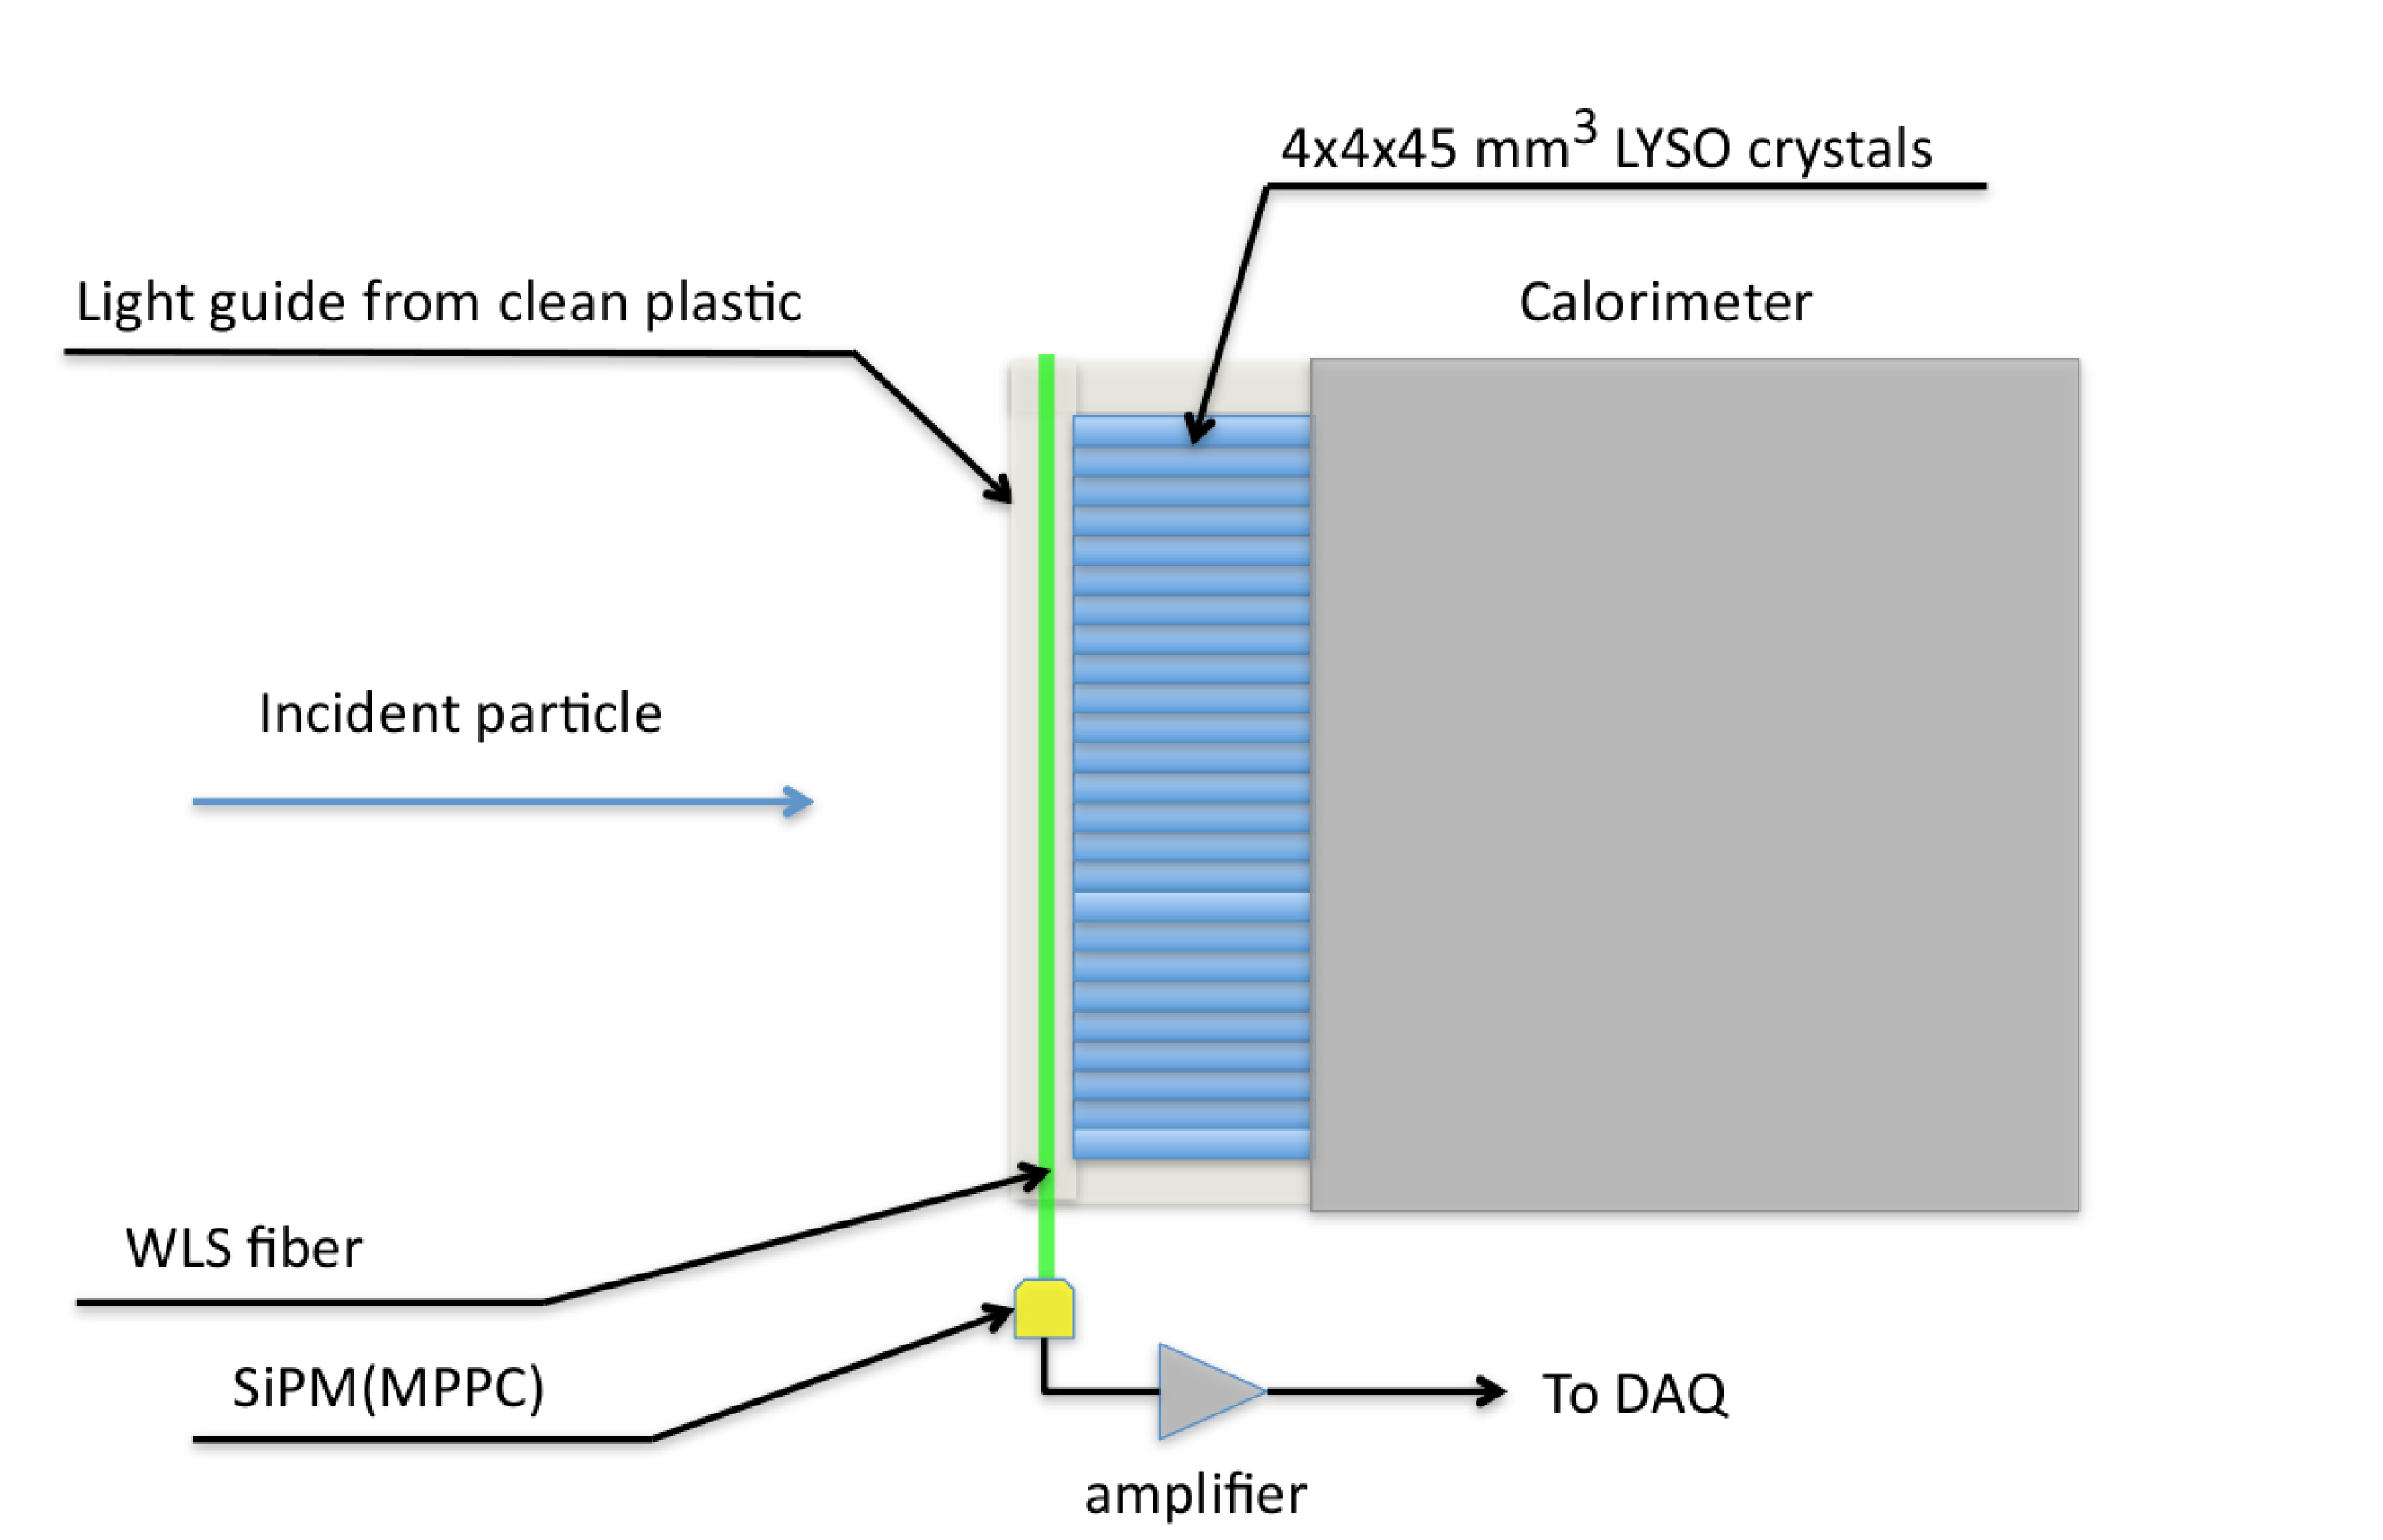
\includegraphics[width=0.98\linewidth]{ps_summary}
\caption{A schematic drawing of the pre-shower calorimeter.}
%
\end{figure}
%
\begin{figure}
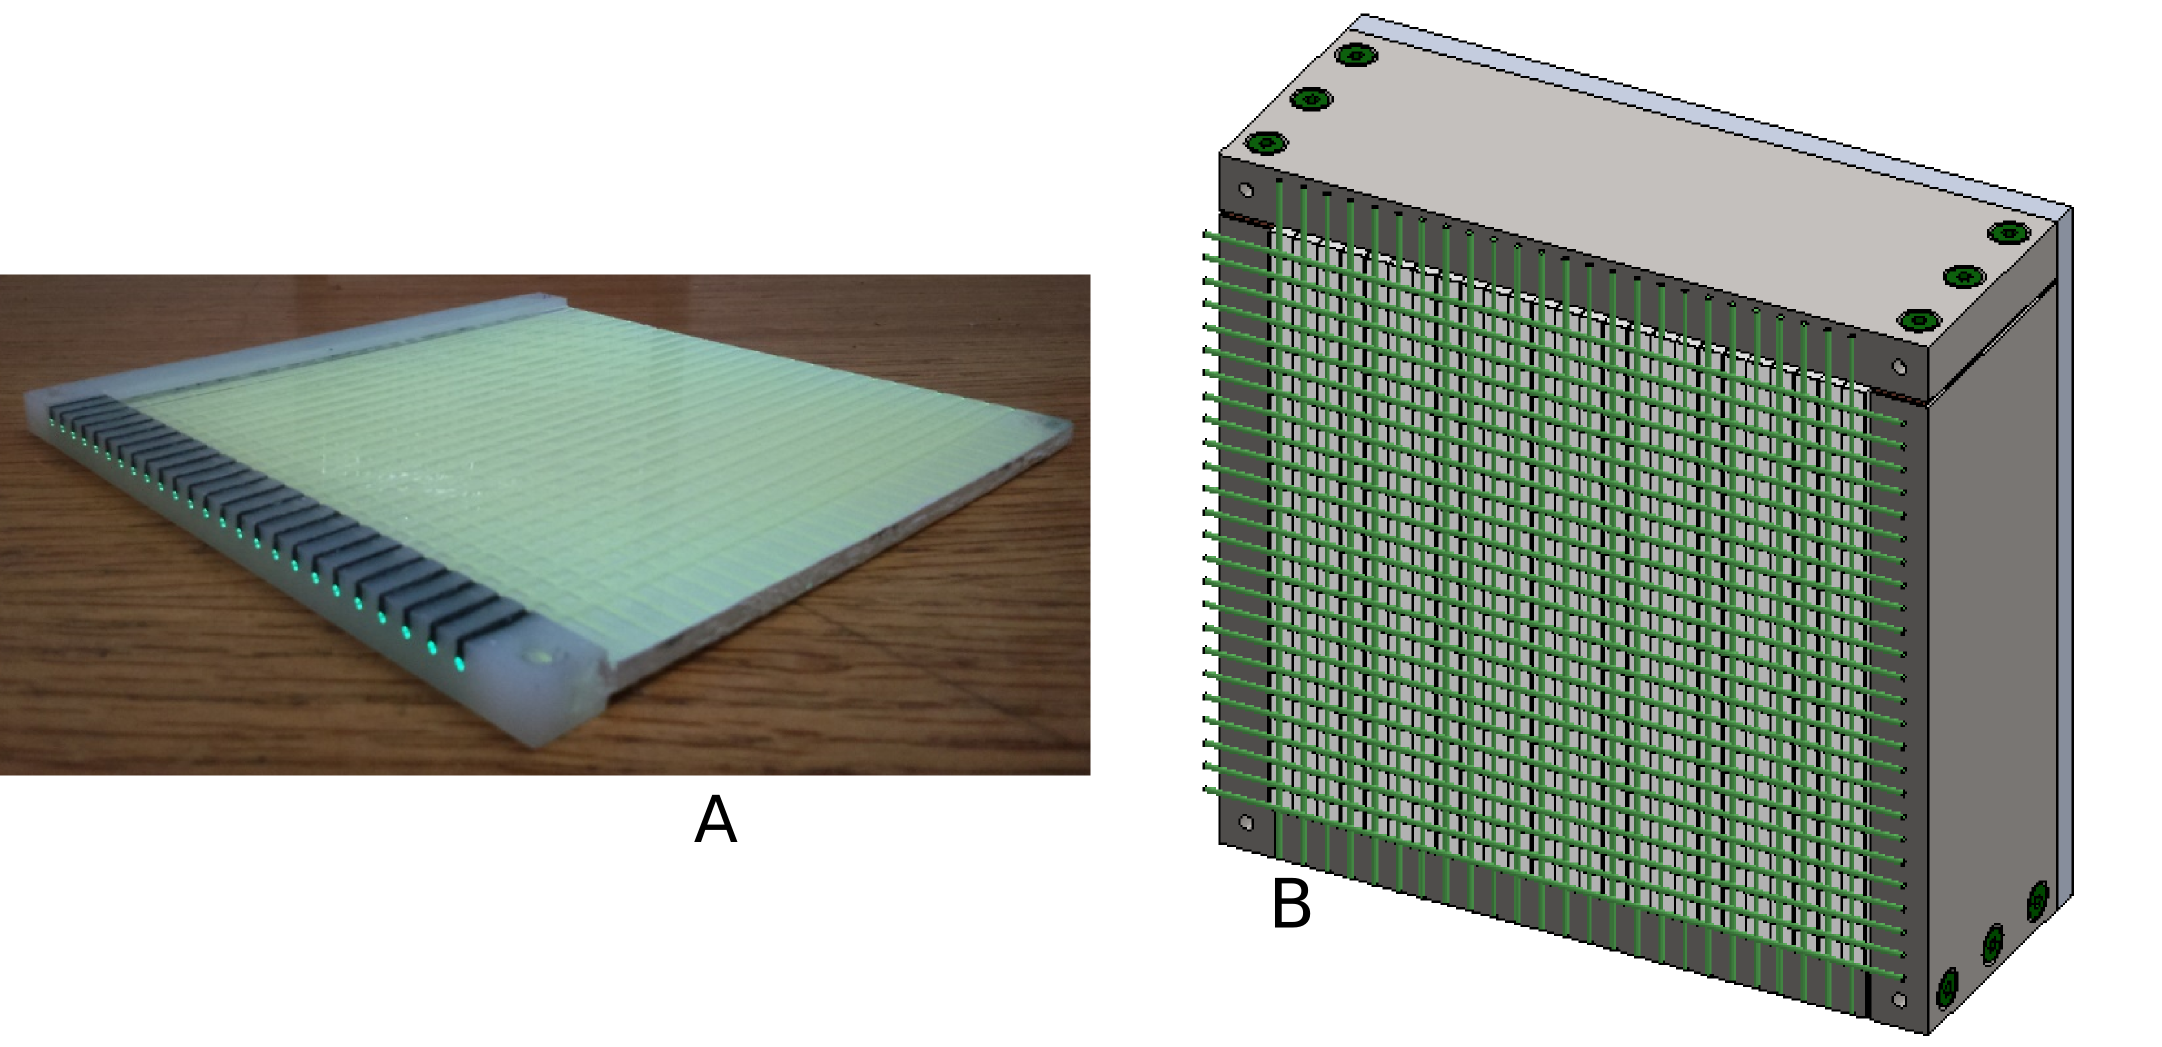
\includegraphics[width=0.98\linewidth]{matrix_wlsf}
\caption{(A) WLSF mounting; (B) Matrix + WLSF;}
\end{figure}
%
\begin{figure}
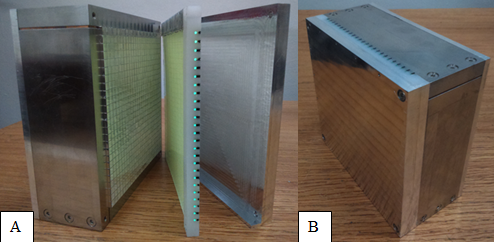
\includegraphics[width=0.98\linewidth]{ps_closing}
\caption{(A) Before closing; (B) Detector Closed;}
\end{figure}
%
The detector consist of a 25x25 matrix of crystals (LYSO). Each crystal has dimensions 4x4x45 (mm) and is covered by a reflector sheet (Vikuiti-ESR de 3M). The reflector was added to it using a thermoformation procedure. The light from the matrix is collected using wavelength shifting fibers (Y11(200)M). The net of fibers was mounted in UVT acrylic. At the end of each WLSF there is small light guide (UVT acrylic) connected to a Multi-pixel photon counter (Hamamatsu S10931-025P) to measure the photons collected.
%
%
\section{Readout}
The readout consist of 50 MPPC distributed into 25 per axis. Each MPPC has its own bias (CAEN A1519B) and its own amplifier. The amplifiers are connected to a QCD (CAEN V792), reading each channel individually.\\
In order to test the performance of the pre-shower the following setup was built:
At the top of the pre-shower there is a Muon detector, bellow the pre-shower there is a small calorimeter and bellow this another Muon detector. The trigger for the acquisition system is generated by a coincidence of the two Muon detectors. In this way the pre-shower was tested using Muons coming from cosmic rays. In order to test the readout, a set of data was collected using different orientations of the pre-shower. A total of 300000 Muons events were analized ( \~ one week of measurements).
\begin{figure}
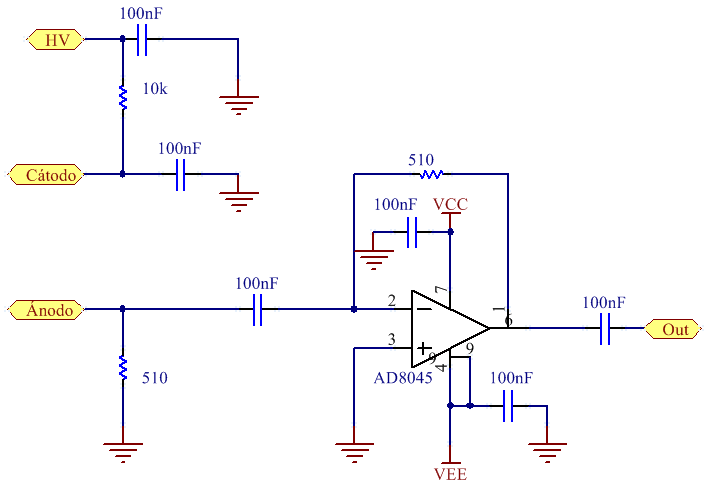
\includegraphics[width=0.98\linewidth]{ps_bias_amp}
\caption{MPPC Bias and amplification circuit.}
%
\end{figure}
%
\begin{figure}
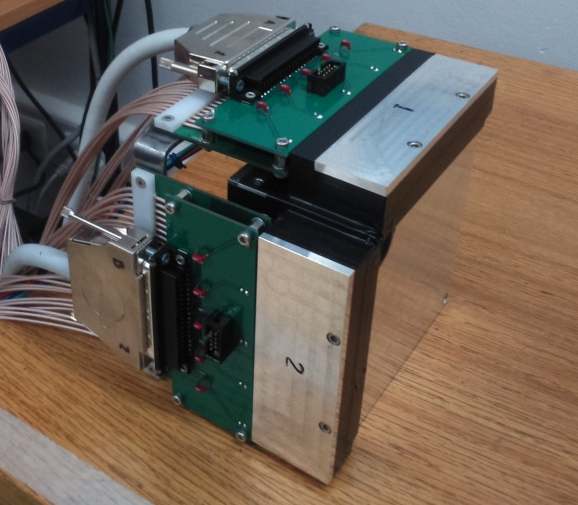
\includegraphics[width=0.98\columnwidth,keepaspectratio]{ps_ready}
\caption{Pre-shower \& Readout finished.}
\end{figure}
%
\begin{figure}
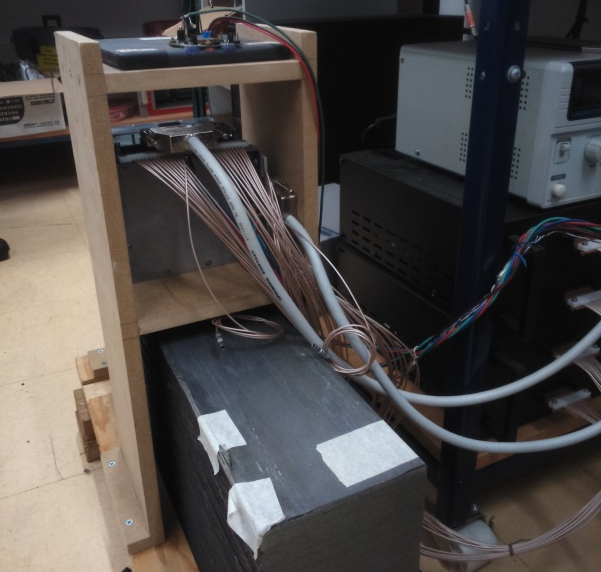
\includegraphics[width=0.98\columnwidth,keepaspectratio]{setup}
\caption{Experimental setup}
\end{figure}
%
\section{Simulations}
A complete simulation of the pre-shower detector has been implemented using Geant4.
\begin{figure}
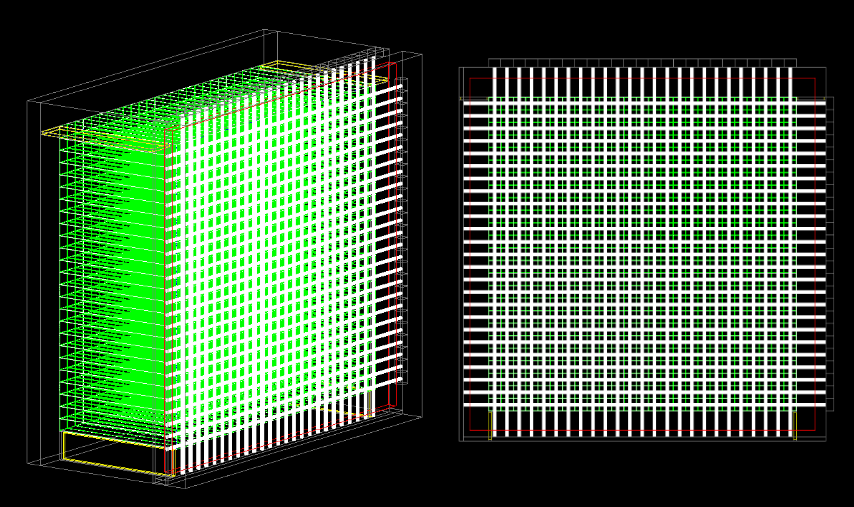
\includegraphics[width=0.98\columnwidth,keepaspectratio]{geometry}
\caption{Full simulation of the pre-shower detector on Geant4.}
\end{figure}
%
Studies on the effect of incident particles on the components of the pre-shower detector has been preformed in order to detect any abnormality. 
%
\begin{figure}
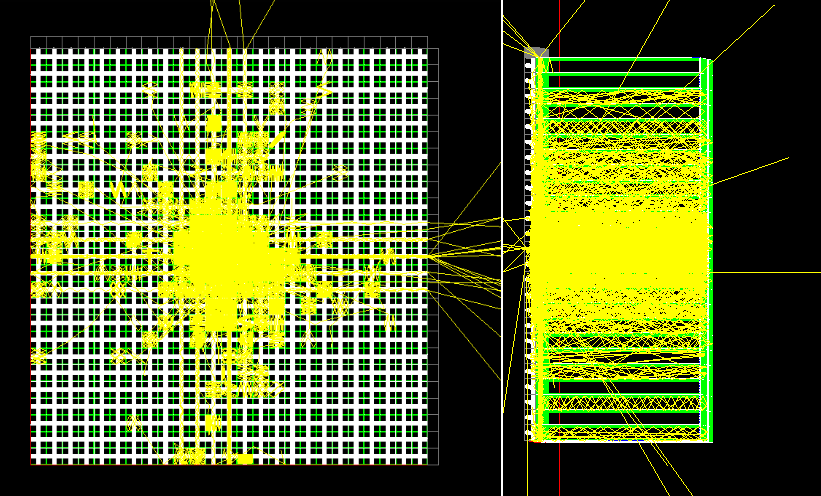
\includegraphics[width=0.98\columnwidth,keepaspectratio]{showers}
\caption{Electromagnetic showers in the pre-shower detector produced by gammas.}
\end{figure}
%
A full reconstruction algorithm has been designed allowing position and energy reconstruction of overlapping electromagnetic showers.
%
\section{Performance}
\begin{figure}
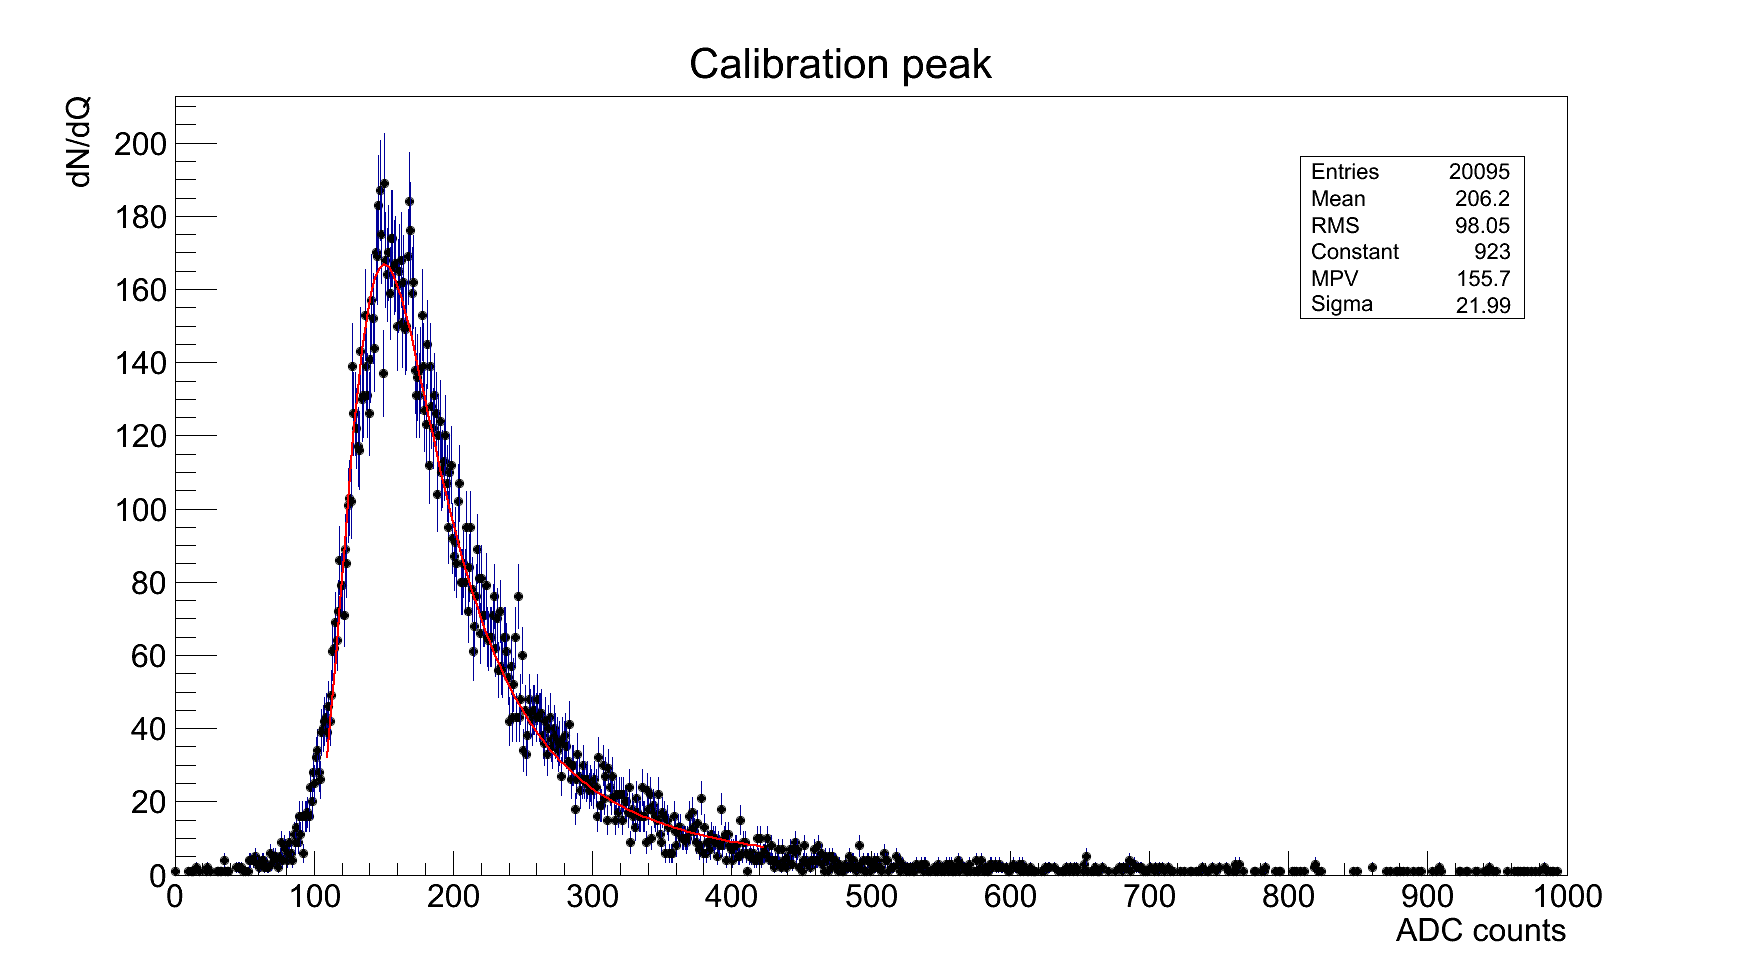
\includegraphics[width=0.98\columnwidth,keepaspectratio]{cal_peak}
\caption{Calibration peak from Landau pdf.}
In order to compare all fibers, a calibration was performed using the MPV of the Landau distribution observed.
\end{figure}
%
\begin{figure}
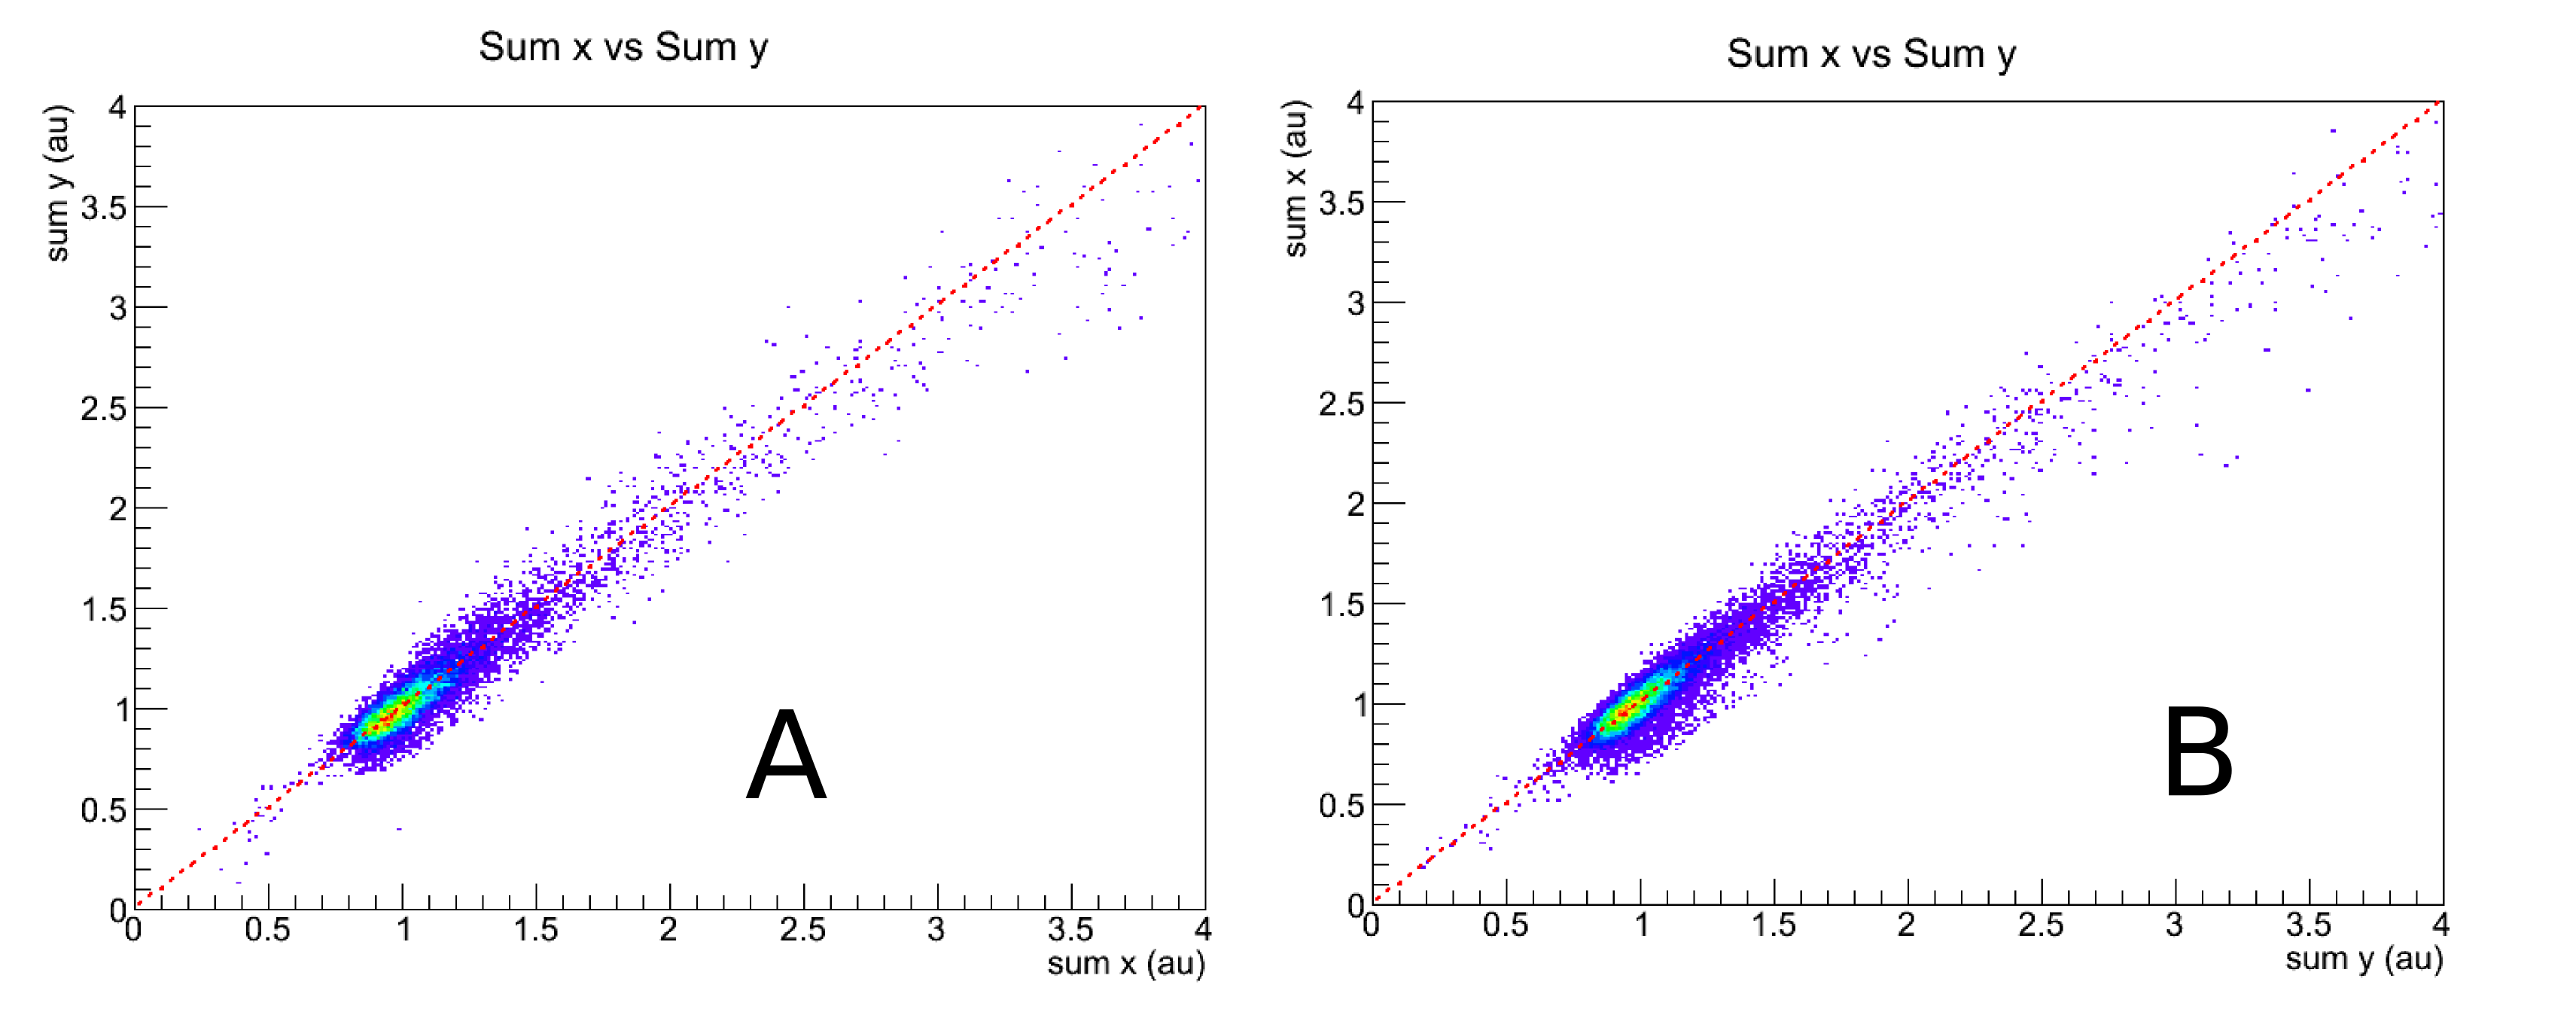
\includegraphics[width=0.98\columnwidth,keepaspectratio]{sumxy_comp}
\caption{Correlation between measurement axes}
\end{figure}
%
\begin{figure}
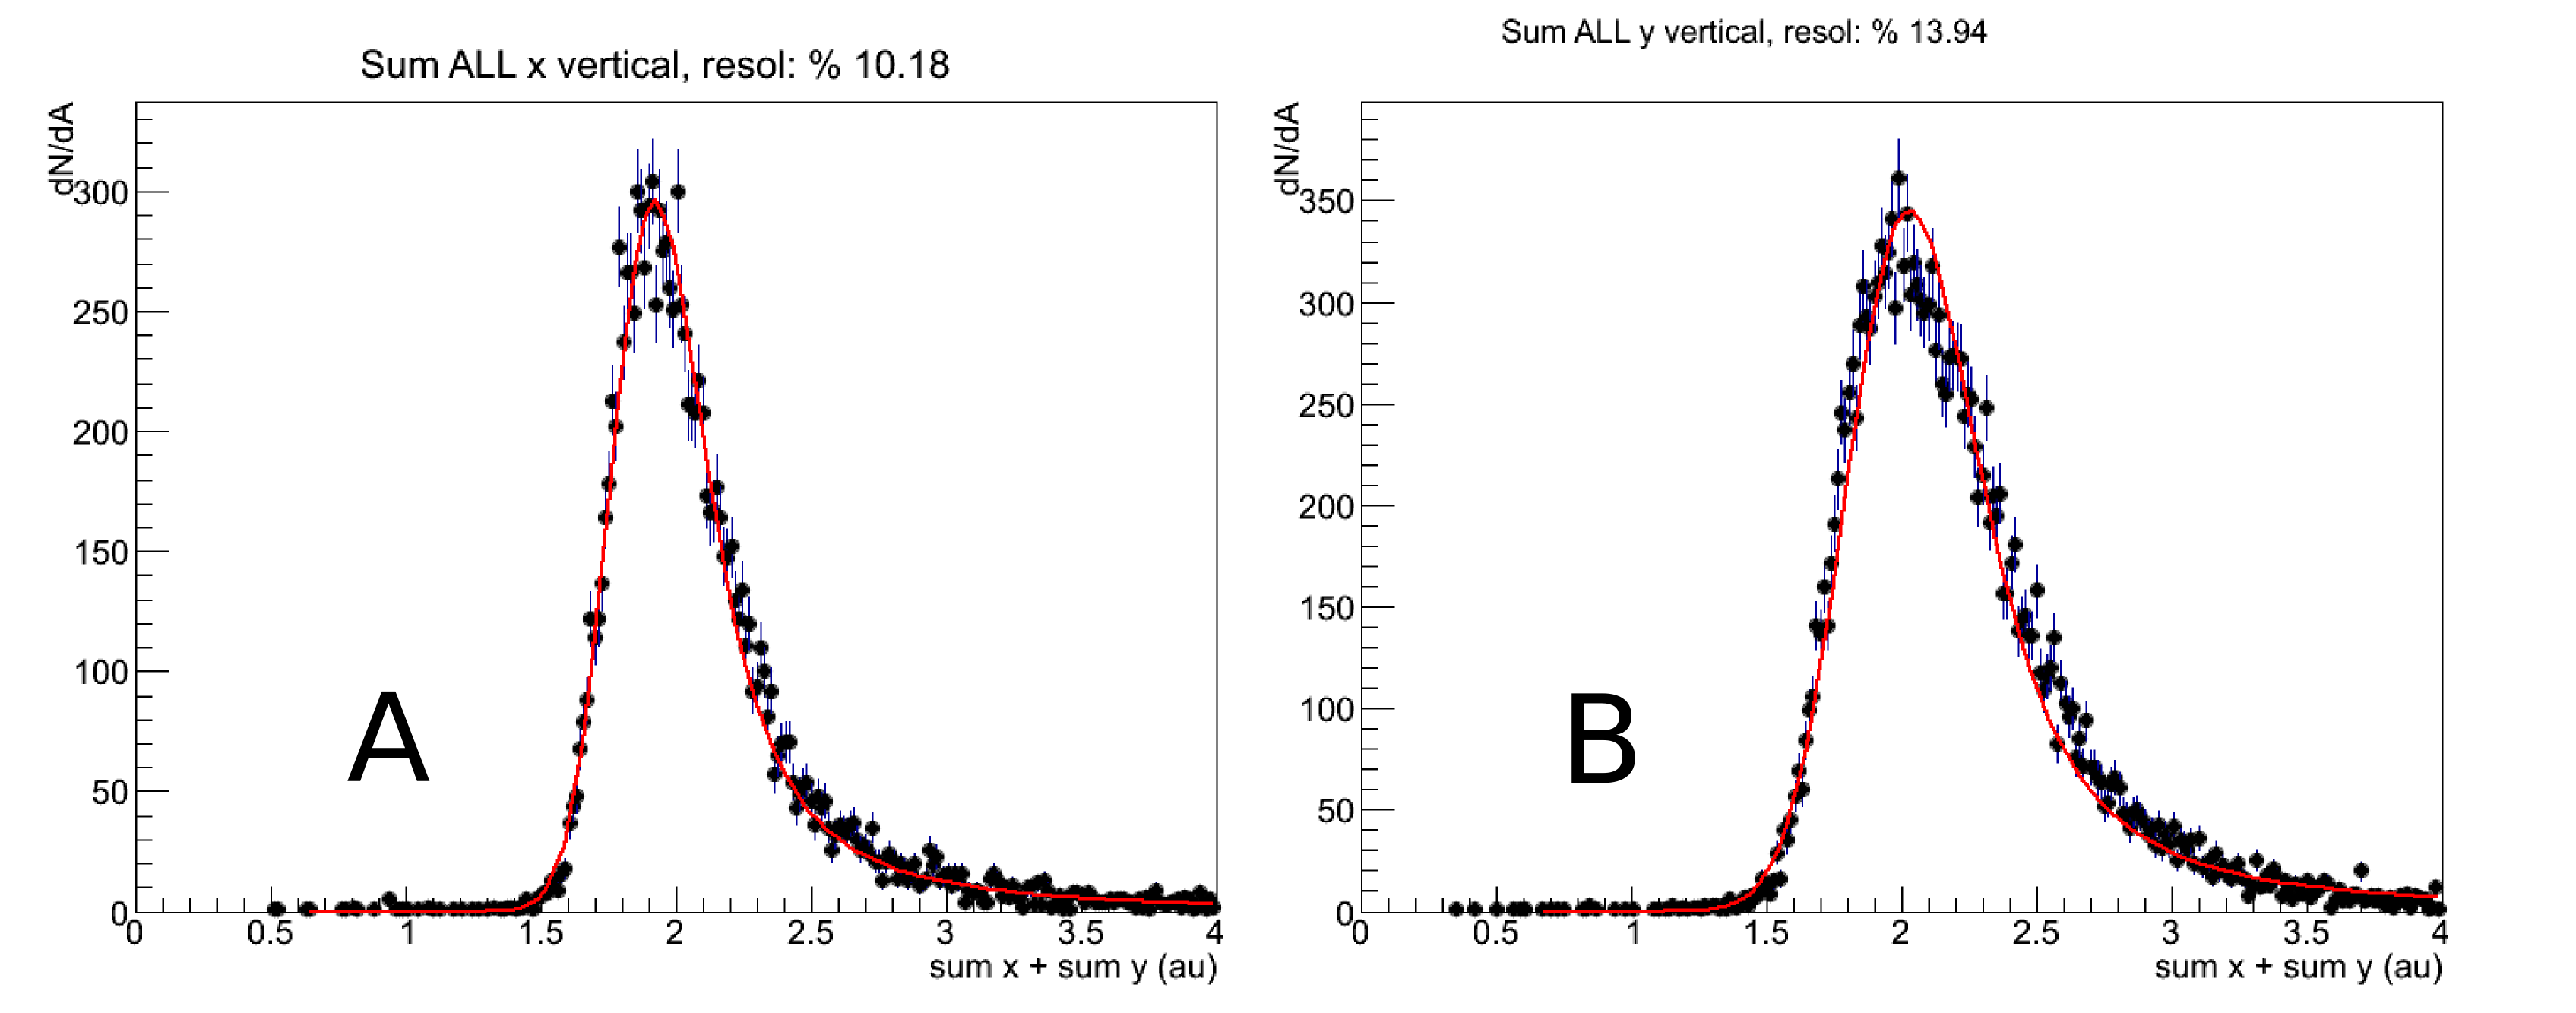
\includegraphics[width=0.98\columnwidth,keepaspectratio]{ps_res}
\caption{Energy resolution. Vertical position on X (A) and Y (B)}
\end{figure}
%
%
%
\section{Conclusions}
\begin{itemize}
\item An efficient procedure of construction of the pre-shower has been created, the studies performed during the construction of the first prototype will allow us to build a new version with improved performance.
\item The first prototype has shown good performance regarding the correlation of energy measurements obtained from the two independent axes, using data collected from cosmic Muons.
\item The full simulation of the pre-shower has been implemented. Initial results has shown improvements in spatial resolution.
\item The reconstruction algorithm for the pre-shower has been designed and tested with simulations. The test against real data will be done in the future.
\end{itemize}
%
\section*{Acknowledgment}
This work was supported by the Chilean BASAL grant FB0821.
Part of this work was done as the undergraduate thesis of Esteban Zambrano.
\nocite{agostinelli2003geant4}
\nocite{preshower_proposal}
%
\section{References}
%For use with external .bib file
% First command removes "References" canned text
% For more info visit: http://www.tex.ac.uk/cgi-bin/texfaq2html?label=fixnam
\bibliographystyle{IEEEtran}
\bibliography{biblio.bib}
%
\end{document}